\documentclass[12pt,letterpaper]{article}
\usepackage[utf8]{inputenc}
\usepackage[spanish]{babel}
\usepackage{graphicx}
\usepackage[left=2cm,right=2cm,top=2cm,bottom=2cm]{geometry}
\usepackage{graphicx} % figuras
% \usepackage{subfigure} % subfiguras
\usepackage{float} % para usar [H]
\usepackage{amsmath}
%\usepackage{txfonts}
\usepackage{stackrel} 
\usepackage{multirow}
\usepackage{enumerate} % enumerados
\renewcommand{\labelitemi}{$-$}
\renewcommand{\labelitemii}{$\cdot$}
% \author{}
% \title{Caratula}
\begin{document}

% Fancy Header and Footer
% \usepackage{fancyhdr}
% \pagestyle{fancy}
% \cfoot{}
% \rfoot{\thepage}
%

% \usepackage[hidelinks]{hyperref} % CREA HYPERVINCULOS EN INDICE

% \author{}
\title{Caratula}

\begin{titlepage}
\begin{center}
\large{UNIVERSIDAD PRIVADA DE TACNA}\\
\vspace*{-0.025in}
\begin{figure}[htb]
\begin{center}

\includegraphics[width=8cm]{./Imagenes/logo}
\end{center}
\end{figure}
\vspace*{0.15in}
INGENIERIA DE SISTEMAS  \\

\vspace*{0.5in}
\begin{large}
TITULO:\\
\end{large}

\vspace*{0.1in}
\begin{Large}
\textbf{Informe Laboratorio Nro 04 Inteligencia de Negocios} \\
\end{Large}

\vspace*{0.3in}
\begin{Large}
\textbf{CURSO:} \\
\end{Large}

\vspace*{0.1in}
\begin{large}
INTELIGENCIA DE NEGOCIOS\\
\end{large}

\vspace*{0.3in}
\begin{Large}
\textbf{DOCENTE(ING):} \\
\end{Large}

\vspace*{0.1in}
\begin{large}
 Patrick Cuadros Quiroga\\
\end{large}

\vspace*{0.2in}
\vspace*{0.1in}
\begin{large}
Integrantes: \\
\begin{flushleft}
COAQUIRA COAQUIRA, Guimer Senon		 \hfill	(2015053226) \\
\end{flushleft}
\end{large}
\end{center}

\end{titlepage}


\tableofcontents % INDICE
\thispagestyle{empty} % INDICE SIN NUMERO
\newpage
\setcounter{page}{1} % REINICIAR CONTADOR DE PAGINAS DESPUES DEL INDICE

\begin{document}

\section{Objetivos}
✓ Realizar el modelamiento dimensional de los ejercicios dados

\section{Requerimientos}
\item{✓ Conocimientos\\
Para el desarrollo de esta práctica se requerirá de los siguientes conocimientos básicos:
- Conocimientos básicos de administración de base de datos Microsoft SQL Server.
- Conocimientos básicos de SQL.\\\\
✓ Software\\
Asimismo se necesita los siguientes aplicativos:
- Microsoft SQL Server 2016 o superior
- Base de datos AdventureWorksDW2016 o superior}

\section{Consideraciones Iniciales}
\item{
✓ Generar todos los modelos fisicos de los diagramas entidad relación y modelo dimensional en bases de datos separadas en Microsoft SQL Server.}

\section{Desarrollo}
\item{
\textbf{Ejercicio N° 01: Envíos}\\\\
El siguiente diagrama E / R simplificado describe el envío de mercancías. Los lotes pertenecientes a ciertos grupos se
envían a ciertos destinos en varios países a través de diferentes modos de transporte. Un cierto centro de costos es
responsable de cada envío. La dimensión de tiempo consiste en mes y año}

\begin{center}
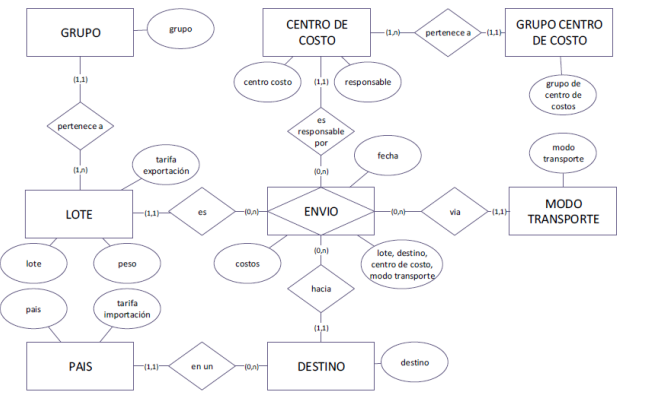
\includegraphics[width=15cm]{./Imagenes/diagrama1}
\end{center}

\begin{center}
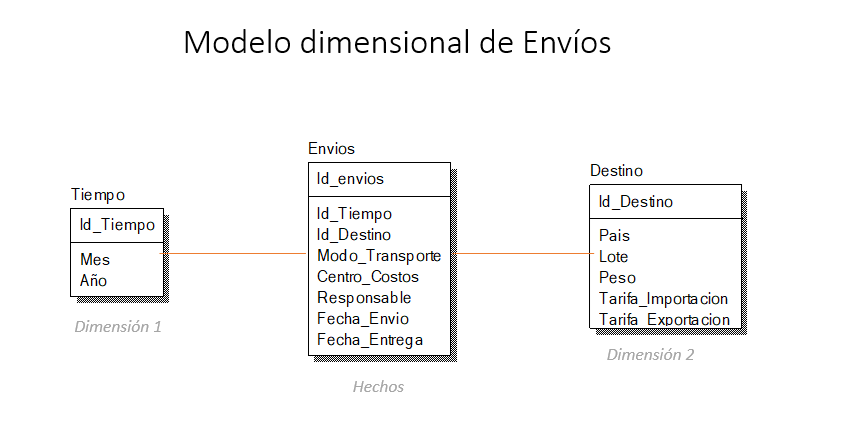
\includegraphics[width=15cm]{./Imagenes/dimension1}
\end{center}

\item{
\textbf{Ejercicio N° 02: Reserva de viajes}\\\\
En este esquema de E / R, un cliente (que es de cierto tipo) reserva un viaje en una agencia de viajes. La agencia de viajes trabaja para un determinado operador turístico. El viaje va a un destino determinado que pertenece a un país determinado.La dimensión de tiempo consiste en mes, trimestre y año

\begin{center}
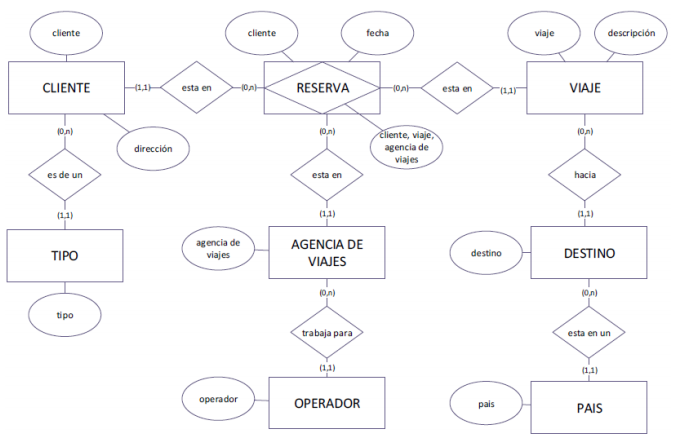
\includegraphics[width=15cm]{./Imagenes/diagrama2}
\end{center}

\begin{center}
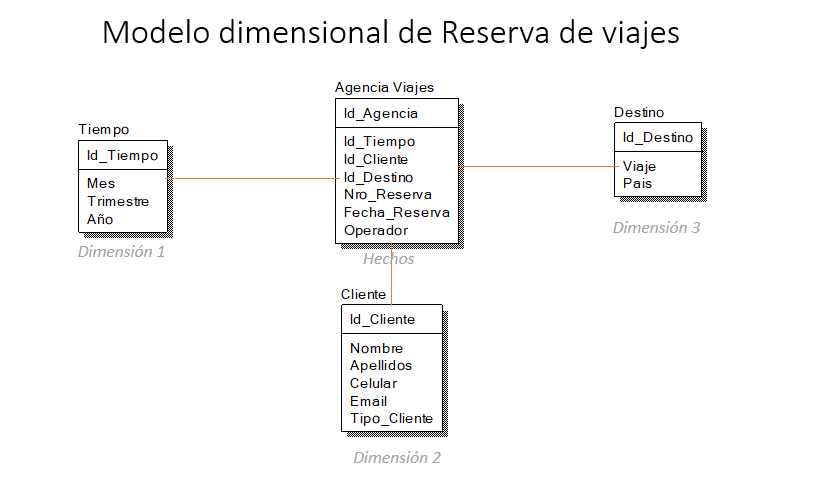
\includegraphics[width=15cm]{./Imagenes/dimension2}
\end{center}

\item{
\textbf{Ejercicio N° 03: Gestion de proyectos}\\\\
Este esquema E / R simplificado muestra un caso gestión del proyecto.
El proyecto para un cliente se divide en varios paquetes de trabajo y siempre una persona es responsable de completar la
tarea. Se cuida en un lugar determinado.
La dimensión de tiempo consiste de día, mes y año.

\begin{center}
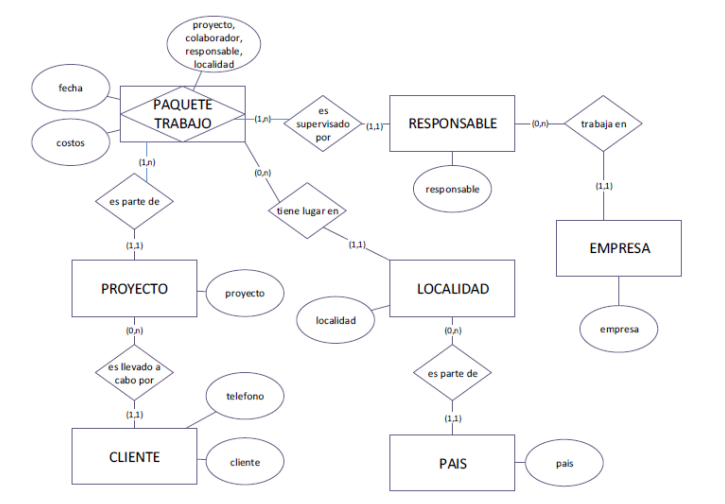
\includegraphics[width=15cm]{./Imagenes/diagrama3}
\end{center}

\begin{center}
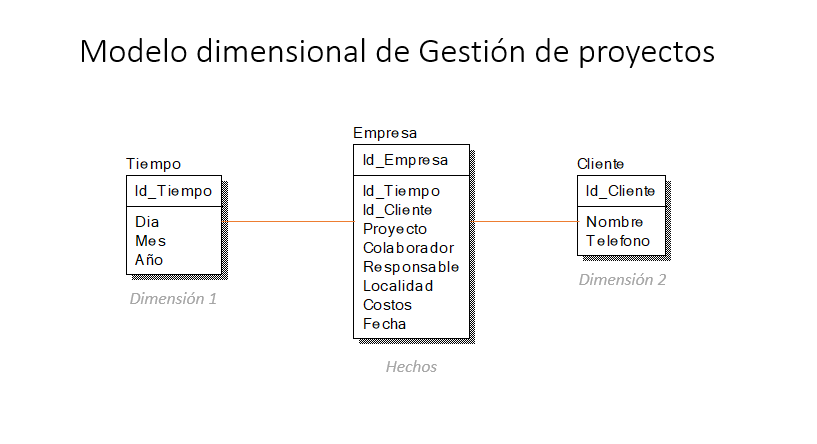
\includegraphics[width=15cm]{./Imagenes/dimension3}
\end{center}

% Bibliografía.
%-----------------------------------------------------------------
\begin{thebibliography}{99}
https://www.isotools.org/2015/02/23/que-es-el-balanced-scorecard-conoce-su-funcionamiento-y-ventajas/\\
https://economipedia.com/definiciones/modelo-canvas.html\\
http://www.infoviews.com.mx/Bitam/ScoreCard/]\\
https://innokabi.com/canvas-de-modelo-de-negocio/\\

\bibitem{Cd94} Autor, \emph{Título}, Revista/Editor, (año)

\end{thebibliography}

\end{document}


\end{document}
